\documentclass[UTF8]{ctexart}
\usepackage{gbt7714} % GB/T 7714 参考文献格式宏包
\usepackage{amsmath} % align package
\usepackage{graphicx} % 图片插入宏包
\usepackage{geometry}       % 调整页面边距
\usepackage{listings} % program listing package
\usepackage{xcolor} % Required for syntax highlighting in listings package
\usepackage{titlesec} % 标题格式宏包
\usepackage{subcaption} % 子图宏包
% 页面边距设置
\geometry{a4paper, margin=1in}
\setlength{\parindent}{0pt} % 设置全局段前缩进为0

% 定义超链接颜色
\usepackage{hyperref}
\hypersetup{
    colorlinks=true,
    linkcolor=blue,
    filecolor=magenta,      
    urlcolor=cyan,
    pdftitle={Overleaf Example},
    pdfpagemode=FullScreen,
}

% 定义文件名格式
\newcommand{\filename}[1]{\texttt{#1}}

% \titleformat{\section}{\raggedright\Large\bfseries}{\thesection}{1em}{}

\lstset{language=Python, % 设置代码语言
    basicstyle=\ttfamily\small, % 设置字体样式
    keywordstyle=\color{blue}, % 设置关键字颜色
    commentstyle=\color{green!50!black}, % 设置注释颜色
    stringstyle=\color{red}, % 设置字符串颜色
    showstringspaces=false, % 不显示字符串中的空格
    numbers=left, % 在左侧显示行号
    numberstyle=\tiny\color{gray}, % 设置行号样式
    breaklines=true, % 自动换行
    breakatwhitespace=true, % 换行只在空格处
    frame=single, % 设置代码框样式
    captionpos=b % 设置标题位置
}

\title{作业 1 \\ Assignment 1}
\author{Computer Vision}
% \date{}

\begin{document}
\maketitle

% 声明作业的相关细则

\section*{重要注意事项 \\ Important Notice}

\begin{enumerate}
    \item 本次作业的提交截止时间为 \textbf{2025 年 3 月 26 日 23:59:59}。请按时在 Canvas 上提交作业。 \\
    The deadline for this assignment is 23:59:59 on March 26, 2025. Please submit the assignment on Canvas on time.
    \item 请将作业的所有文件打包成一个压缩文件,命名为 \filename{学号-姓名-作业编号},例如\filename{12345678-张三-Assignment01.zip}。 \\
    Please pack all the files of the assignment into a compressed file, named as \filename{StudentID - Name - AssignmentNumber}, for example, \filename{12345678-ZhangSan-Assignment01.zip}.
    \item 请包含一份\textbf{pdf}格式的报告,报告中包含你的姓名、学号、作业编号、各个任务所要求的内容。如任务有代码实现,请将代码文件也包含在压缩文件中。 \\
    Please include a report in \textbf{pdf} format, which contains your name, student ID, assignment number, and the requirements of each task. If the task requires code implementation, please include the code file in the compressed file.
\end{enumerate}

\section{任务 1 \quad Task 1}

\subsection{问题1 \quad Question 1}
假如你现在是一个摄影师,现在烈日当空,你的相机或者手机屏幕亮度非常糟糕,慌忙之中,你拍摄了下面这张照片,如图 \ref{fig:Fuji_light} 所示。 \\
Suppose you are a photographer, and now the sun is blazing. Your camera or phone screen brightness is very poor. In a hurry, you took the following photo, as shown in Figure \ref{fig:Fuji_light}.

\begin{figure}[h]
    \centering
    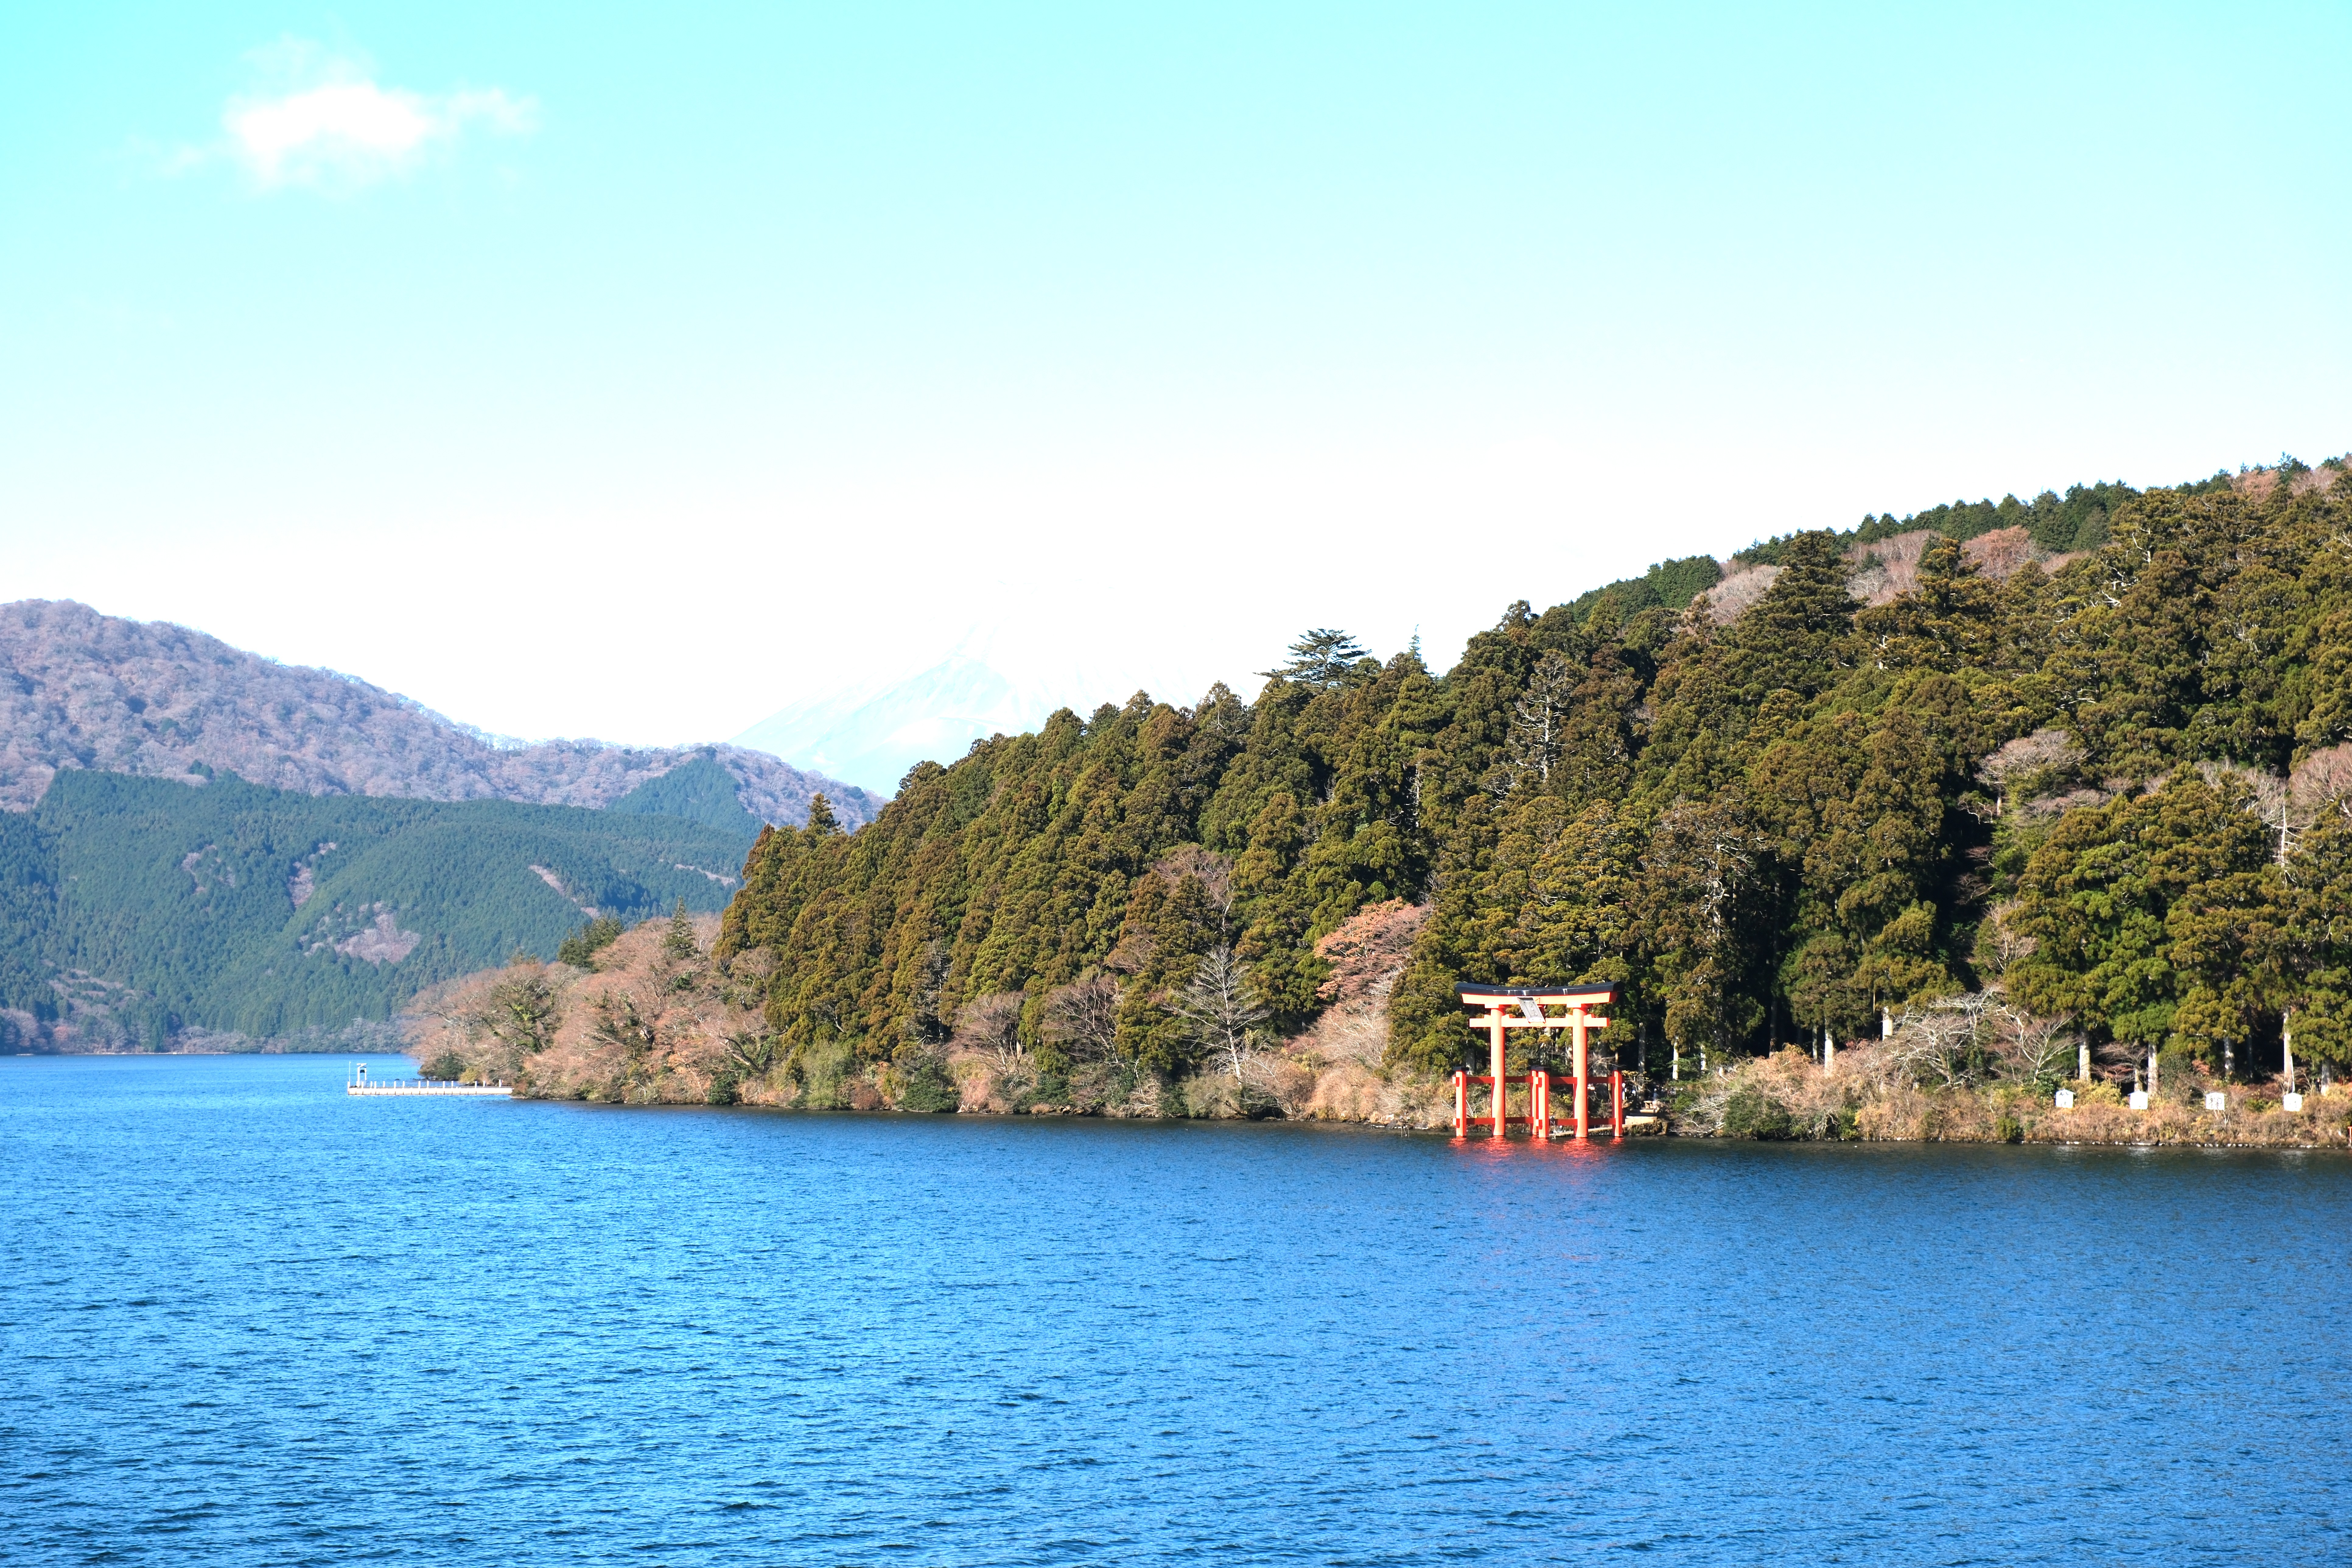
\includegraphics[width=0.5\textwidth]{image/Fuji_light.JPG}
    \caption{水中鸟居与富士山? \quad Torii in the Water and Mount Fuji?}
    \label{fig:Fuji_light}
\end{figure}

请你回答以下问题: \\
Please answer the following questions:
\begin{enumerate}
    \item 你认为这张照片的曝光度是不是有问题?如果有问题,你认为是什么问题? \\
    Do you think there is a problem with the exposure of this photo? If there is a problem, what do you think the problem is?
    \item 有没有这么一个工具可以显示在你的屏幕上,能够帮助你判断照片的曝光度是否正确?请简述如何使用这个工具。[提示:直方图] \\
    Is there a tool that can be displayed on your screen to help you determine if the exposure of the photo is correct? Please describe how to use this tool. (Hint: Histogram)
\end{enumerate}

\subsection{代码任务 \quad Code Task}
图 \ref{fig:star} 是一张助教拍摄的夜晚的天空。但是助教并不是想数星星,而是在意当天晚上的天气,但是助教眼睛不太好使,请你帮助他。 \\
Figure \ref{fig:star} is a photo of the night sky taken by the teaching assistant. However, the teaching assistant is not interested in counting stars but in the weather that night. However, the teaching assistant's eyesight is not very good, please help him.

\begin{figure}[h]
    \centering
    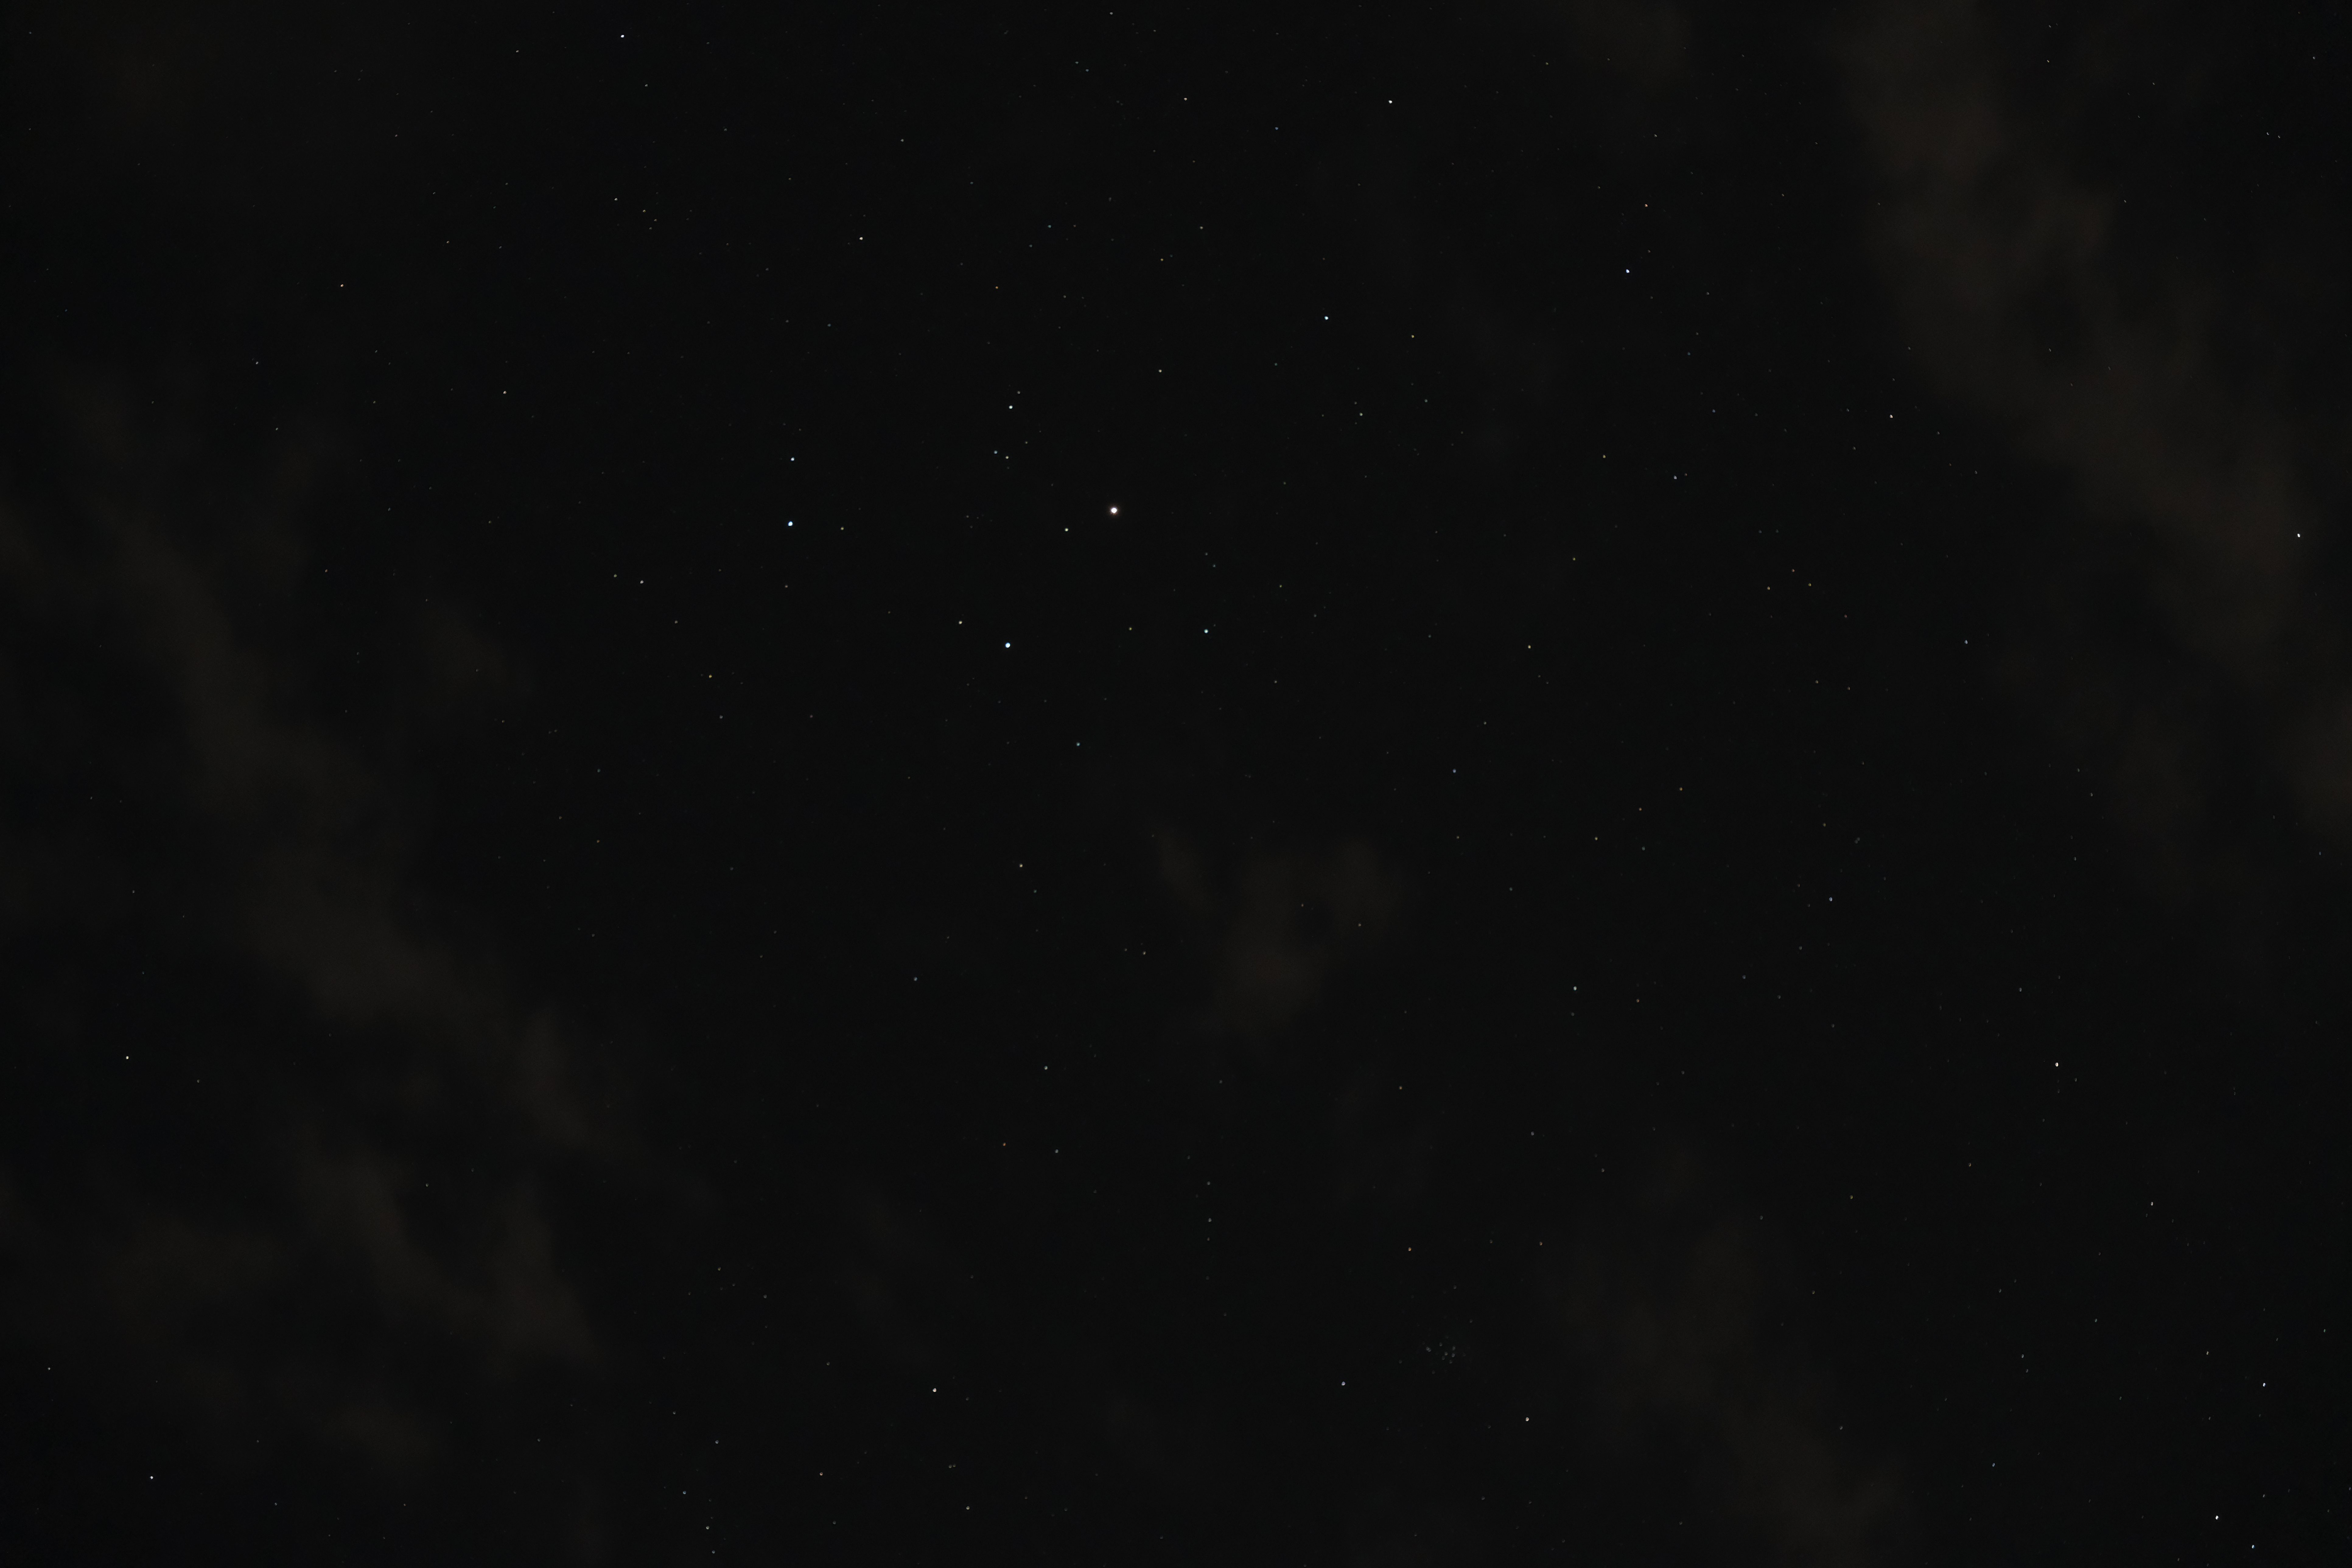
\includegraphics[width=0.5\textwidth]{image/star.JPG}
    \caption{夜晚的天空 \quad Night Sky}
    \label{fig:star}
\end{figure}


请你编写代码,完成以下任务: \\
Please write code to complete the following tasks:
\begin{enumerate}
    \item 读取这张图片。图片原文件见附件 \filename{star.jpg}。 \\
    Read this image. The original file of the image is attached as \filename{star.jpg}.
    \item 将这张图片转换为灰度图像。 \\
    Convert this image to a grayscale image.
    \item 计算并绘制这张图片的直方图。 \\
    Calculate and draw the histogram of this image.
    \item 对这张图片进行直方图均衡化。 \\
    Perform histogram equalization on this image.
    \item 计算并绘制均衡化后的图片的直方图。 \\
    Calculate and draw the histogram of the equalized image.
    \item 保存或显示均衡化后的图片。 \\
    Save or display the equalized image.
\end{enumerate}

请在报告中展示你的过程和结果。所有的编程语言和库都可以接受,包括但不限于 Python、C++、MATLAB 等。 \\
Please show your process and results in the report. All programming languages and libraries are acceptable, including but not limited to Python, C++, MATLAB, etc.

\subsection{问题 2 \quad Question 2}

最后请回答以下问题: \\
Finally, please answer the following questions:
\begin{enumerate}
    \item 根据你的理解,简述直方图均衡化的原理。 \\
    Based on your understanding, briefly describe the principle of histogram equalization.
    \item 直方图均衡化前后图像和直方图分别发生了什么变化? \\
    What changes have occurred in the image and histogram before and after histogram equalization?
    \item 你认为在什么情况下直方图均衡化是有用的? \\
    In what situations do you think histogram equalization is useful?
    \item 从直方图均衡化后的图像来看,对于那个夜晚的天气,请你给出你的判断,并给出有力的理由。 \\
    From the perspective of the histogram-equalized image, please give your judgment on the weather that night and provide strong reasons.
\end{enumerate}

\section{任务 2 \quad Task 2}

\subsection{问题1 \quad Question 1}

假设你现在是一名车牌识别系统开发者,负责对路面车辆的车牌进行特征提取。在实际场景中,车牌图像虽然拍摄较为清晰,但可能仍会受到部分噪声干扰。虽然当今基于深度学习的方法已经很成熟了,但今天你降智了,只能使用传统图像处理方法。 \\
Suppose you are a license plate recognition system developer responsible for extracting features from license plates of road vehicles. In actual scenarios, although the license plate images are relatively clear, they may still be affected by some noise. Although deep learning-based methods are mature today, you are not smart today and can only use traditional image processing methods.

\begin{figure}
    \centering
    \begin{subfigure}[b]{0.45\textwidth}
        \centering
        \includegraphics[width=\textwidth]{image/LP13.jpg}
        \caption{车牌图像 1 \quad License Plate Image 1}
        \label{fig:plate1}
    \end{subfigure}
    \hfill
    \begin{subfigure}[b]{0.45\textwidth}
        \centering
        \includegraphics[width=\textwidth]{image/LP14.jpg}
        \caption{车牌图像 2 \quad License Plate Image 2}
        \label{fig:plate2}
    \end{subfigure}
    \caption{经典中国蓝色车牌 \quad Classic Chinese Blue License Plate}
    \label{fig:plate}
\end{figure}

对于车牌识别的第一步,你需要找到图片中的车牌,这需要你通过边缘检测来提取车牌的特征。请你回答以下问题: \\
For the first step of license plate recognition, you need to find the license plate in the image, which requires you to extract the features of the license plate through edge detection. Please answer the following questions:
\begin{enumerate}
    \item 你认为,车牌有什么有别于其他区域的显著特征? \\
    What significant features do you think distinguish the license plate from other regions?
    \item 你认为,根据车牌的特征,哪种边缘检测算子更适合提取车牌的边缘特征? \\
    Based on the features of the license plate, which edge detection operator do you think is more suitable for extracting the edge features of the license plate?
    \item 你认为,图像中的那些元素会对边缘检测造成干扰?会对车牌特征提取造成什么影响?有什么方法可以减轻这些干扰? \\
    What elements in the image do you think will interfere with edge detection? What impact will they have on license plate feature extraction? What methods can be used to mitigate these interferences?
\end{enumerate}

\subsection{代码任务 \quad Code Task}

如图 \ref{fig:plate3} 所示,是一张车辆的图像,车牌区域相对清晰。
你需要通过边缘检测提取车牌特征,为后续的字符识别做准备,同时尽可能减少环境噪声的影响。
图 \ref{fig:plate4} 是理论上最理想的效果,显然这是不可能的,但你需要尽可能接近这个效果。 \\
As shown in Figure \ref{fig:plate3}, it is an image of a vehicle, and the license plate area is relatively clear. You need to extract the license plate features through edge detection to prepare for subsequent character recognition while minimizing the impact of environmental noise as much as possible. Figure \ref{fig:plate4} shows the theoretically ideal effect, which is obviously impossible, but you need to get as close to this effect as possible.

\begin{figure}
    \centering
    \begin{subfigure}[b]{0.45\textwidth}
        \centering
        \includegraphics[width=\textwidth]{image/LP11.jpg}
        \caption{待处理图像 \quad Image to be Processed}
        \label{fig:plate3}
    \end{subfigure}
    \hfill
    \begin{subfigure}[b]{0.45\textwidth}
        \centering
        \includegraphics[width=\textwidth]{image/canny_center.jpg}
        \caption{目标效果 \quad Target Effect}
        \label{fig:plate4}
    \end{subfigure}
    \caption{代码任务图像 \quad Code Task Image}
\end{figure}

请你编写代码,完成以下任务:\\
Please write code to complete the following tasks: 
\begin{enumerate} 
    \item 读取这张图像。图片原文件见附件 \filename{plate.jpg}。\\
    Read the image.  The original file of the image is attached as \filename{plate.jpg}.
    \item 将图像大小调整为 $400 \times 300$ 。\\
    Resize the image to $400 \times 300$.
    \item 将图像转换为灰度图像。\\
    Convert the image to grayscale. 
    \item 对灰度图像应用不同的边缘检测算子(例如 Sobel、Canny、Laplacian),分别提取车牌区域的边缘特征。请尽可能尝试各种你认为合适的边缘检测算子以及参数。\\
    Apply different edge detection operators (e.g., Sobel, Canny, Laplacian) to the grayscale image to extract the edge features of the license plate area. Please try various edge detection operators and parameters that you think are appropriate.
    \item (可选,但建议)根据需要对边缘检测结果进行适当的预处理和后处理(例如使用高斯滤波降噪、形态学操作增强边缘连贯性),以尽可能排除环境噪声的干扰。\\
    (Optional, but recommended)
    Perform appropriate preprocessing (e.g., Gaussian filtering for noise reduction) and postprocessing (e.g., morphological operations to enhance edge continuity) on the edge maps to minimize interference from environmental noise. 
    \item 显示或保存各边缘检测方法的结果,便于比较和分析。\\
    Display or save the results of each edge detection method for comparison and analysis. 
\end{enumerate}

请在报告中展示你的代码实现过程、实验结果以及各边缘检测方法在车牌特征提取任务中的对比分析。\\
Please include in your report the implementation process, experimental results, and comparative analysis of each edge detection method for license plate feature extraction.

\subsection{问题 2 \quad Question 2}

最后,请回答以下问题:\\
Finally, please answer the following questions: 
\begin{enumerate} 
    \item 你在使用 Sobel、Canny 和 Laplacian 算子提取车牌特征时,观察到了哪些主要差异?\\
    What are the main differences you observed among the edge maps produced by the Sobel, Canny, and Laplacian operators when extracting license plate features? 
    \item 环境噪声如何影响边缘检测在车牌特征提取中的表现?你采用了哪些方法来降低噪声干扰,并取得了怎样的效果?\\
    How does environmental noise affect the performance of edge detection in license plate feature extraction, and what methods did you use to reduce the noise? What results did you achieve? 
    \item 根据你的实验结果,哪种边缘检测方法在本次车牌特征提取任务中表现最佳?请说明理由,并讨论该方法可能的局限性。\\
    Based on your experimental results, which edge detection method performed best in this license plate feature extraction task? Please explain your reasons and discuss any potential limitations of this method. 
    \item (可选)你认为,除了本次任务关注的车牌边缘特征外,还有哪些其他特征可能对车牌识别有帮助?\\
    (Optional) In addition to the license plate edge features focused on in this task, what other features do you think might be helpful for license plate recognition?
\end{enumerate}

\section*{评分标准 \\ Grading Criteria}
\begin{itemize}
    \item 40\%:任务 1 \quad Task 1
    \begin{itemize}
        \item 20\%:问题 1 \quad Question 1
        \item 50\%:代码任务 \quad Code Task
        \item 30\%:问题 2 \quad Question 2
    \end{itemize}
    \item 40\%:任务 2 \quad Task 2
    \begin{itemize}
        \item 20\%:问题 1 \quad Question 1
        \item 50\%:代码任务 \quad Code Task
        \item 30\%:问题 2 \quad Question 2
    \end{itemize}
    \item 20\%:报告质量 \quad Report Quality
\end{itemize}

\section*{提示 \\ Tips}
\begin{itemize}
    \item 再一次声明,所有的编程语言和库都可以接受,包括但不限于 Python、C++、MATLAB 等。 \\
    Once again, all programming languages and libraries are acceptable, including but not limited to Python, C++, MATLAB, etc.
    \item 请在报告中展示你的过程和结果。 \\
    Please show your process and results in the report.
    \item 所有的问题都是开放性问题,答案不唯一。 回答问题即有 80\% 的分数,剩下的 20\% 的分数取决于你的创新、见解和分析。 \\ 
    All questions are open-ended, and there is no unique answer. Answering the questions accounts for 80\% of the score, and the remaining 20\% depends on your innovation, insights, and analysis.
    \item 鼓励使用大语言模型进行辅助来完成作业。但请谨慎使用,避免出现答案雷同导致的成绩扣分。 \\
    It is encouraged to use LLMs for assistance in completing the task. But please use it carefully to avoid score deduction due to similar answers.
    \item 对于所有的问题,我们更加关注你的个人思考、分析、见解和创新。 必要时,可以进行重点突出强调,例如:\textbf{加粗}、“我认为”字样等。 \\
    For all questions, we pay more attention to your personal thinking, analysis, insights, and innovation. When necessary, you can emphasize it, such as bold, "I think", etc.
    \item 报告语言和形式不限,但为了整洁美观,建议使用 \LaTeX{} 或 Markdown 进行撰写。 \\
    The language and form of the report are not limited, but for neatness and beauty, it is recommended to use \LaTeX{} or Markdown for writing.
    \item 你无需担忧本次作业所出现图片的版权问题,因为这些图片都是由助教拍摄的。 \\
    You don't need to worry about the copyright issues of the images in this assignment, because these images are all taken by the teaching assistant.
\end{itemize}

\end{document}
